\section{Programowanie AI i GitHub Copilot w Visual Studio Code}

\subsection{Wprowadzenie}
GitHub Copilot to asystent programisty wykorzystujący sztuczną inteligencję (AI) do generowania kodu, sugerowania rozwiązań, tworzenia komentarzy i automatyzowania pracy w środowisku Visual Studio Code (VS Code). Opiera się na dużych modelach językowych (LLM) wytrenowanych na kodzie źródłowym z GitHuba i publicznych repozytoriów.

\subsection{Tryb Agent Mode}
W trybie \textbf{Agent Mode} Copilot działa jak inteligentny współprogramista. Użytkownik może wydawać mu polecenia w języku naturalnym, a agent samodzielnie wykonuje operacje, np.:
\begin{itemize}
    \item generowanie plików i klas,
    \item kompilowanie i uruchamianie projektu,
    \item tworzenie testów jednostkowych,
    \item wykonywanie zadań administracyjnych (np. Git, CI/CD),
    \item analizowanie błędów i sugerowanie poprawek.
\end{itemize}

Agenty mogą pracować w tle, komunikować się przez \textit{Copilot Chat}, a także wykonywać proste zadania autonomicznie, np. „stwórz endpoint API dla klasy \texttt{Product}”.

\subsection{Różnice między klasycznym Copilotem a Agent Mode}
\begin{itemize}
    \item \textbf{Klasyczny Copilot} – podpowiada linie lub bloki kodu na podstawie kontekstu w edytorze.
    \item \textbf{Agent Mode} – działa jak interaktywny chatbot, który rozumie intencje użytkownika, może wywoływać komendy, analizować pliki projektu i działać w wielu krokach.
\end{itemize}

\subsection{Bezpieczeństwo: Allow i Deny List}
Aby uniknąć ryzyka wykonania niepożądanych poleceń systemowych, Agent Mode korzysta z list:
\begin{itemize}
    \item \textbf{Allow List} – lista komend, które agent może wykonać (np. \texttt{dotnet build}, \texttt{dotnet test}).
    \item \textbf{Deny List} – komendy, które są blokowane (np. \texttt{rm -rf}, \texttt{sudo}).
\end{itemize}

Administrator lub użytkownik może te listy konfigurować lokalnie w ustawieniach VS Code.

\subsection{Limity zapytań i kontrola wydajności}
W ustawieniach Copilota można ustawić:
\begin{itemize}
    \item \textbf{Max Requests} – maksymalną liczbę równoległych zapytań do modelu,
    \item \textbf{Response Timeout} – czas oczekiwania na odpowiedź.
\end{itemize}
W projektach zespołowych pozwala to uniknąć spowolnień i nadmiernego zużycia zasobów API.

\subsection{Copilot Instructions i konwencje kodowania}
Copilot może generować kod zgodny z przyjętymi standardami:
\begin{itemize}
    \item \texttt{PascalCase} dla klas i metod,
    \item \texttt{camelCase} dla zmiennych,
    \item komentarze XML i dokumentacja metod.
\end{itemize}
Można też dopisać własne instrukcje w pliku \texttt{.copilot.json}, np.:
\begin{lstlisting}[language=json, caption={Przykład konfiguracji Copilota w JSON}]
{
  "style": "use PascalCase for classes, camelCase for variables",
  "language": "C#",
  "comment_format": "XML"
}
\end{lstlisting}

\subsection{Tryby czatu i personalizacja}
Copilot pozwala przełączać tzw. \textbf{Chat Modes}, które zmieniają styl i ton pracy agenta:
\begin{itemize}
    \item \texttt{Default Mode} – standardowy styl pomocy,
    \item \texttt{Beast Mode} – agresywne sugestie optymalizacji,
    \item \texttt{Explain Mode} – tłumaczenie działania kodu linia po linii.
\end{itemize}

\subsection{Snooze Completions – wstrzymanie podpowiedzi}
Użytkownik może czasowo wyłączyć podpowiedzi AI, jeśli pracuje nad kodem manualnie lub nie chce rozproszeń.  
Przykład: „Snooze for 10 minutes” – wstrzymuje automatyczne uzupełnianie przez 10 minut.

\subsection{Coding Agents i GitHub Actions}
Copilot integruje się z GitHub Actions, co pozwala automatyzować procesy CI/CD:
\begin{itemize}
    \item testowanie i budowanie projektu po zatwierdzeniu PR,
    \item analiza błędów i propozycje poprawek w pipeline,
    \item automatyczne generowanie dokumentacji i changelogów.
\end{itemize}

Agent może np. po wykonaniu komendy \texttt{commit} zaproponować opis PR i wygenerować testy do nowych metod.

\subsection{Statystyki użycia i analiza produktywności}
Copilot rejestruje dane o efektywności (lokalnie, bez wysyłania kodu):
\begin{itemize}
    \item liczba akceptowanych sugestii,
    \item średnia długość wygenerowanego kodu,
    \item czas reakcji modelu.
\end{itemize}

Z raportów wynika, że średnio 46–55\% kodu w projektach C\# i TypeScript generowanych z pomocą Copilota jest akceptowane przez programistów.

\subsection{Diagram działania agenta Copilot}
\begin{center}
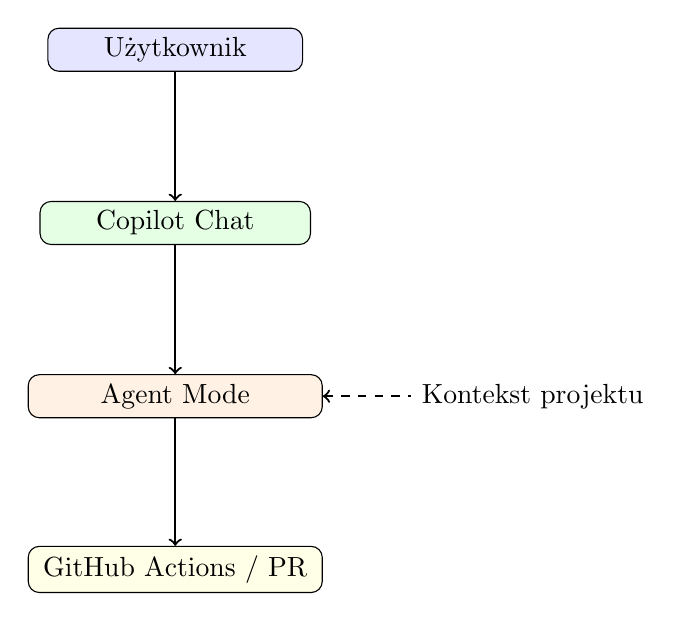
\begin{tikzpicture}[node distance=2.2cm, every node/.style={align=center}]
\node (user) [draw, rounded corners, fill=blue!10, text width=3cm] {Użytkownik};
\node (chat) [draw, rounded corners, fill=green!10, text width=3.2cm, below of=user] {Copilot Chat};
\node (agent) [draw, rounded corners, fill=orange!10, text width=3.5cm, below of=chat] {Agent Mode};
\node (actions) [draw, rounded corners, fill=yellow!10, text width=3.5cm, below of=agent] {GitHub Actions / PR};

\draw[->, thick] (user) -- (chat);
\draw[->, thick] (chat) -- (agent);
\draw[->, thick] (agent) -- (actions);
\draw[<-, thick, dashed] (agent) -- ++(3,0) node[right]{Kontekst projektu};
\end{tikzpicture}
\end{center}

\subsection{MCP (Model Context Protocol) Auto Start}
MCP to protokół rozszerzający możliwości Copilota o dodatkowe źródła kontekstu i narzędzia.

\begin{itemize}
	\item \textbf{Rola MCP} -- dostarcza Copilotowi dodatkowe informacje z zewnętrznych źródeł (bazy danych, API, dokumentacja),
	\item \textbf{Konfiguracja} -- Auto Start mode: \texttt{always}, \texttt{ask}, \texttt{never},
	\item \textbf{Serwery MCP} -- rozszerzenia dostarczające kontekst (np. dostęp do lokalnej dokumentacji projektu),
	\item \textbf{Zarządzanie} -- Extensions → MCP servers w VS Code.
\end{itemize}

\textbf{Przykład użycia:}
\begin{itemize}
	\item MCP może automatycznie dostarczać Copilotowi aktualną dokumentację API projektu,
	\item Umożliwia dostęp do niestandardowych narzędzi deweloperskich (linters, formattery),
	\item Pozwala na integrację z bazą wiedzy zespołu.
\end{itemize}

\subsection{Background Agents i sesje w tle}
Background Agents pozwalają na delegowanie długotrwałych zadań do wykonania w tle, podczas gdy programista kontynuuje pracę.

\begin{itemize}
	\item \textbf{Agent Sessions (UI integration)} -- panel w VS Code pokazujący aktywne sesje agentów,
	\item \textbf{Przypisywanie zadań} -- można utworzyć issue w GitHub i przypisać je do Copilota,
	\item \textbf{Automatyczne PR} -- agent tworzy pull request z rozwiązaniem w tle,
	\item \textbf{Kontynuacja pracy} -- programista może pracować lokalnie, podczas gdy agent działa równolegle.
\end{itemize}

\textbf{Przykładowy workflow:}
\begin{enumerate}
	\item Programista tworzy issue: "Dodać skeleton loading na stronie logowania",
	\item Przypisuje issue do Copilota,
	\item Agent tworzy nowy branch, implementuje rozwiązanie,
	\item Tworzy pull request do review,
	\item Programista przegląda i akceptuje/modyfikuje.
\end{enumerate}

\subsection{Task Lists (To-Do w czacie)}
Copilot może generować listy kroków (task lists) dla złożonych zadań i śledzić ich realizację.

\textbf{Przykład:}
\begin{lstlisting}[caption={Polecenie w Copilot Chat}]
	Użytkownik: "Dodaj stronę z formularzem kontaktowym"
	
	Copilot generuje:
	[ ] Utworzyć nowy plik ContactPage.xaml
	[ ] Dodać pola: Imię, Email, Wiadomość
	[ ] Utworzyć ViewModel z walidacją
	[ ] Dodać endpoint API POST /api/contact
	[ ] Dodać nawigację do strony kontaktu
\end{lstlisting}

Podczas pracy Copilot automatycznie oznacza wykonane kroki:
\begin{itemize}
	\item [x] Utworzyć nowy plik ContactPage.xaml
	\item [x] Dodać pola: Imię, Email, Wiadomość
	\item [ ] Utworzyć ViewModel z walidacją (w trakcie)
\end{itemize}

\subsection{Custom Chat Modes -- Beast Mode}
Beast Mode to przykład niestandardowego trybu czatu, który agresywnie optymalizuje kod.

\textbf{Konfiguracja w projekcie:}
\begin{enumerate}
	\item Utwórz katalog \texttt{.github/chat-modes/}
	\item Utwórz plik \texttt{beast.json}:
\end{enumerate}

\begin{lstlisting}[language=json, caption={Przykład konfiguracji Beast Mode}]
	{
		"name": "Beast Mode",
		"description": "Agresywna optymalizacja kodu",
		"instructions": [
		"Zawsze sugeruj najbardziej wydajne rozwiązanie",
		"Używaj async/await dla operacji I/O",
		"Optymalizuj pod kątem pamięci i procesora",
		"Sugeruj LINQ zamiast pętli where możliwe"
		]
	}
\end{lstlisting}

\textbf{Użycie:} W Copilot Chat wybierz tryb "Beast Mode" i poproś o optymalizację kodu.

\subsection{Podsumowanie rozdziału}
\begin{itemize}
    \item Copilot umożliwia pracę w trybie interaktywnym i autonomicznym.
    \item Agent Mode pozwala wykonywać operacje w środowisku VS Code.
    \item System zapewnia bezpieczeństwo dzięki Allow/Deny List.
    \item Integracja z GitHub Actions umożliwia automatyzację CI/CD.
    \item Wydajność można kontrolować przez limity zapytań.
\end{itemize}

\subsection{Pytania kontrolne}
\begin{enumerate}
    \item Czym różni się klasyczny Copilot od trybu Agent Mode?
    \item Jak działa lista Allow/Deny i dlaczego jest istotna?
    \item Jakie są przykłady integracji Copilota z GitHub Actions?
    \item Jak można ograniczyć liczbę zapytań do modelu?
    \item W jaki sposób Copilot wspiera standardy nazewnictwa w C\#?
\end{enumerate}
